\scanpage{11}
\mspage{2bis}
% archive sheet number: 11

\uline{Cor. 3} Soit $X\unsure{\gtrless|\bowtie}Y$. Alors
\[
X\unsure{\,\cdot\,}\ll Y\ \Longleftrightarrow\ X\leq Y
\]
\deleted{En effet,} On applique cor 1 avec $Z=X$.

\uline{Proposition 3.} \deleted{Supposons} $X\overset{\circ}{\ll}Y\overset{\circ}{\ll}Z$ \deleted{$\unsure{\Longleftrightarrow}$}\inserted{implique} $X\overset{\circ}{\ll}Z$.
\[
\deleted{\Longleftrightarrow\ X\overset{\circ}{\ll}Y\text{ et }Y\overset{\circ}{\ll}Z}
\]
\deleted{a) Supposons $X\overset{\circ}{\ll}Y$ et $Y\overset{\circ}{\ll}Z$, prouvons $X\overset{\circ}{\ll}Z$, i.e. $X\ll Z'\leq Z\Longrightarrow Z'=Z$. \unsure{Comme}}

Par $\unsure{\mathrm{Mog}|\mathrm{Mag}}\,2$ $\exists\,Z'$ \unsure{avec} $X\overset{\circ}{\ll}Z'\leq Z$, \deleted{\unsure{on a|où}} \deleted{\unsure{par Mog}} prouvons $Z'=Z$. Sinon, par Mog 4 on aurait $Z'\mathrel{|\unsure{\circ|0}|}Z$, et par Mog 3 b) $X\mathrel{|\circ|}Z$, d'autre part

\diagram{\begin{tikzcd}[ampersand replacement=\&,column sep=small,row sep=small]
X\arrow[r,phantom,"\overset{\circ}{\ll}"{description}]\arrow[dr,phantom,"\overset{\circ}{\ll}"{description,rotate=-45}]\&Y\arrow[r,phantom,"\overset{\circ}{\ll}"{description}]\&Z\arrow[dl,phantom,"\leq"{description,rotate=45}]\\
\&Z'\&
\end{tikzcd}}

par Mog 3 b) cela implique $X\mathrel{|\circ|}Y$ puisque $Y\overset{\circ}{\ll}Z$, puis $X\mathrel{|\circ|}X$ puisque $X\overset{\circ}{\ll}Y$, \deleted{d'où $X\mid$} mais $X\mathrel{|\circ|}X$ contredit Mog 3 a).

\deleted{\unsure{b)}}\inserted{NB} Supposons \inserted{$X\ll Y\ll Z$ et} $X\overset{\circ}{\ll}Z$. Alors $Y\overset{\circ}{\ll}Z$, car si on avait $Y\ll Z'\unsure{<|\leq}Z$, on en conclurait $X\ll Z'<Z$, contrairement à $X\overset{\circ}{\ll}Z$. \deleted{\unsure{Prouvons}} \deleted{par} Mais on n'a pas \unsure{néc\textsuperscript{t}} $X\overset{\circ}{\ll}Y$, \unsure{exple}.

\figure{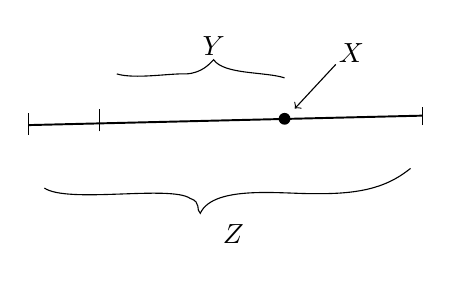
\begin{tikzpicture}[x=1cm,y=1cm]
\draw[line width=.7pt] (0,0)--(5,.12);
\draw (0,-.12)--(0,.15) (.9,-.08)--(.9,.2) (5,0)--(5,.23);
\fill (3.25,.08) circle (.075);
\draw (1.12,.65) .. controls (1.35,.58) and (1.8,.66) .. (2,.65) .. controls (2.2,.66) and (2.3,.78) .. (2.35,.83) .. controls (2.48,.64) and (3,.68) .. (3.25,.6);
\node at (2.35,1) {$Y$};
\draw[->] (3.9,.77)--(3.38,.21);
\node at (4.1,.91) {$X$};
\draw (.2,-.8) .. controls (.5,-1) and (1.8,-.76) .. (2.05,-.93) .. controls (2.2,-.98) and (2.12,-1.08) .. (2.18,-1.12) .. controls (2.35,-.75) and (3.25,-.88) .. (3.65,-.87) .. controls (4.3,-.88) and (4.6,-.75) .. (4.85,-.55);
\node at (2.6,-1.38) {$Z$};
\end{tikzpicture}}

\uline{Cas des figures}

\uline{Prop 1}.F a) $F\gtrless G$ sym. \unsure{réfl.}

b) $F\gtrless G$, $F'\leq F$, $G'\leq G\Longrightarrow F'\gtrless G'$

\uline{Prop \unsure{2|?}}.F Si $F\gtrless G$, \deleted{\unsure{Prop}} alors $F\ll G\Longleftrightarrow F\leq G$

\uline{Cor} Dans l'ens \unsure{de|des} $\unsure{\mathrm{Ssfig}(F)|\mathrm{Ssfi}_0(F)}$, $\ll$ et $\leq$ coïncident
